\section{Autorisation d'usage de l'IA par l'\'el\`eve}
\label{app:ia}

%% Consignes §6.2.2 : « Cette autorisation se trouve en annexe du dossier et
%% doit obligatoirement etre fournie dans le rapport. »
%% Le formulaire vierge compose en LaTeX a ete remplace par le scan du document
%% signe le 25 aout 2026 : Images/autorisation_ia_signee.png

The form of Annexe~7 was completed and signed by the company tutor on 25 August 2026. The
use of generative AI tools is authorised, under the restriction written by hand on the form,
\emph{\foreignlanguage{french}{encadr\'e par la convention ALTEN sur l'utilisation de l'IA}}:
within the scope of ALTEN's internal convention on the use of AI.

\begin{figure}[H]
    \centering
    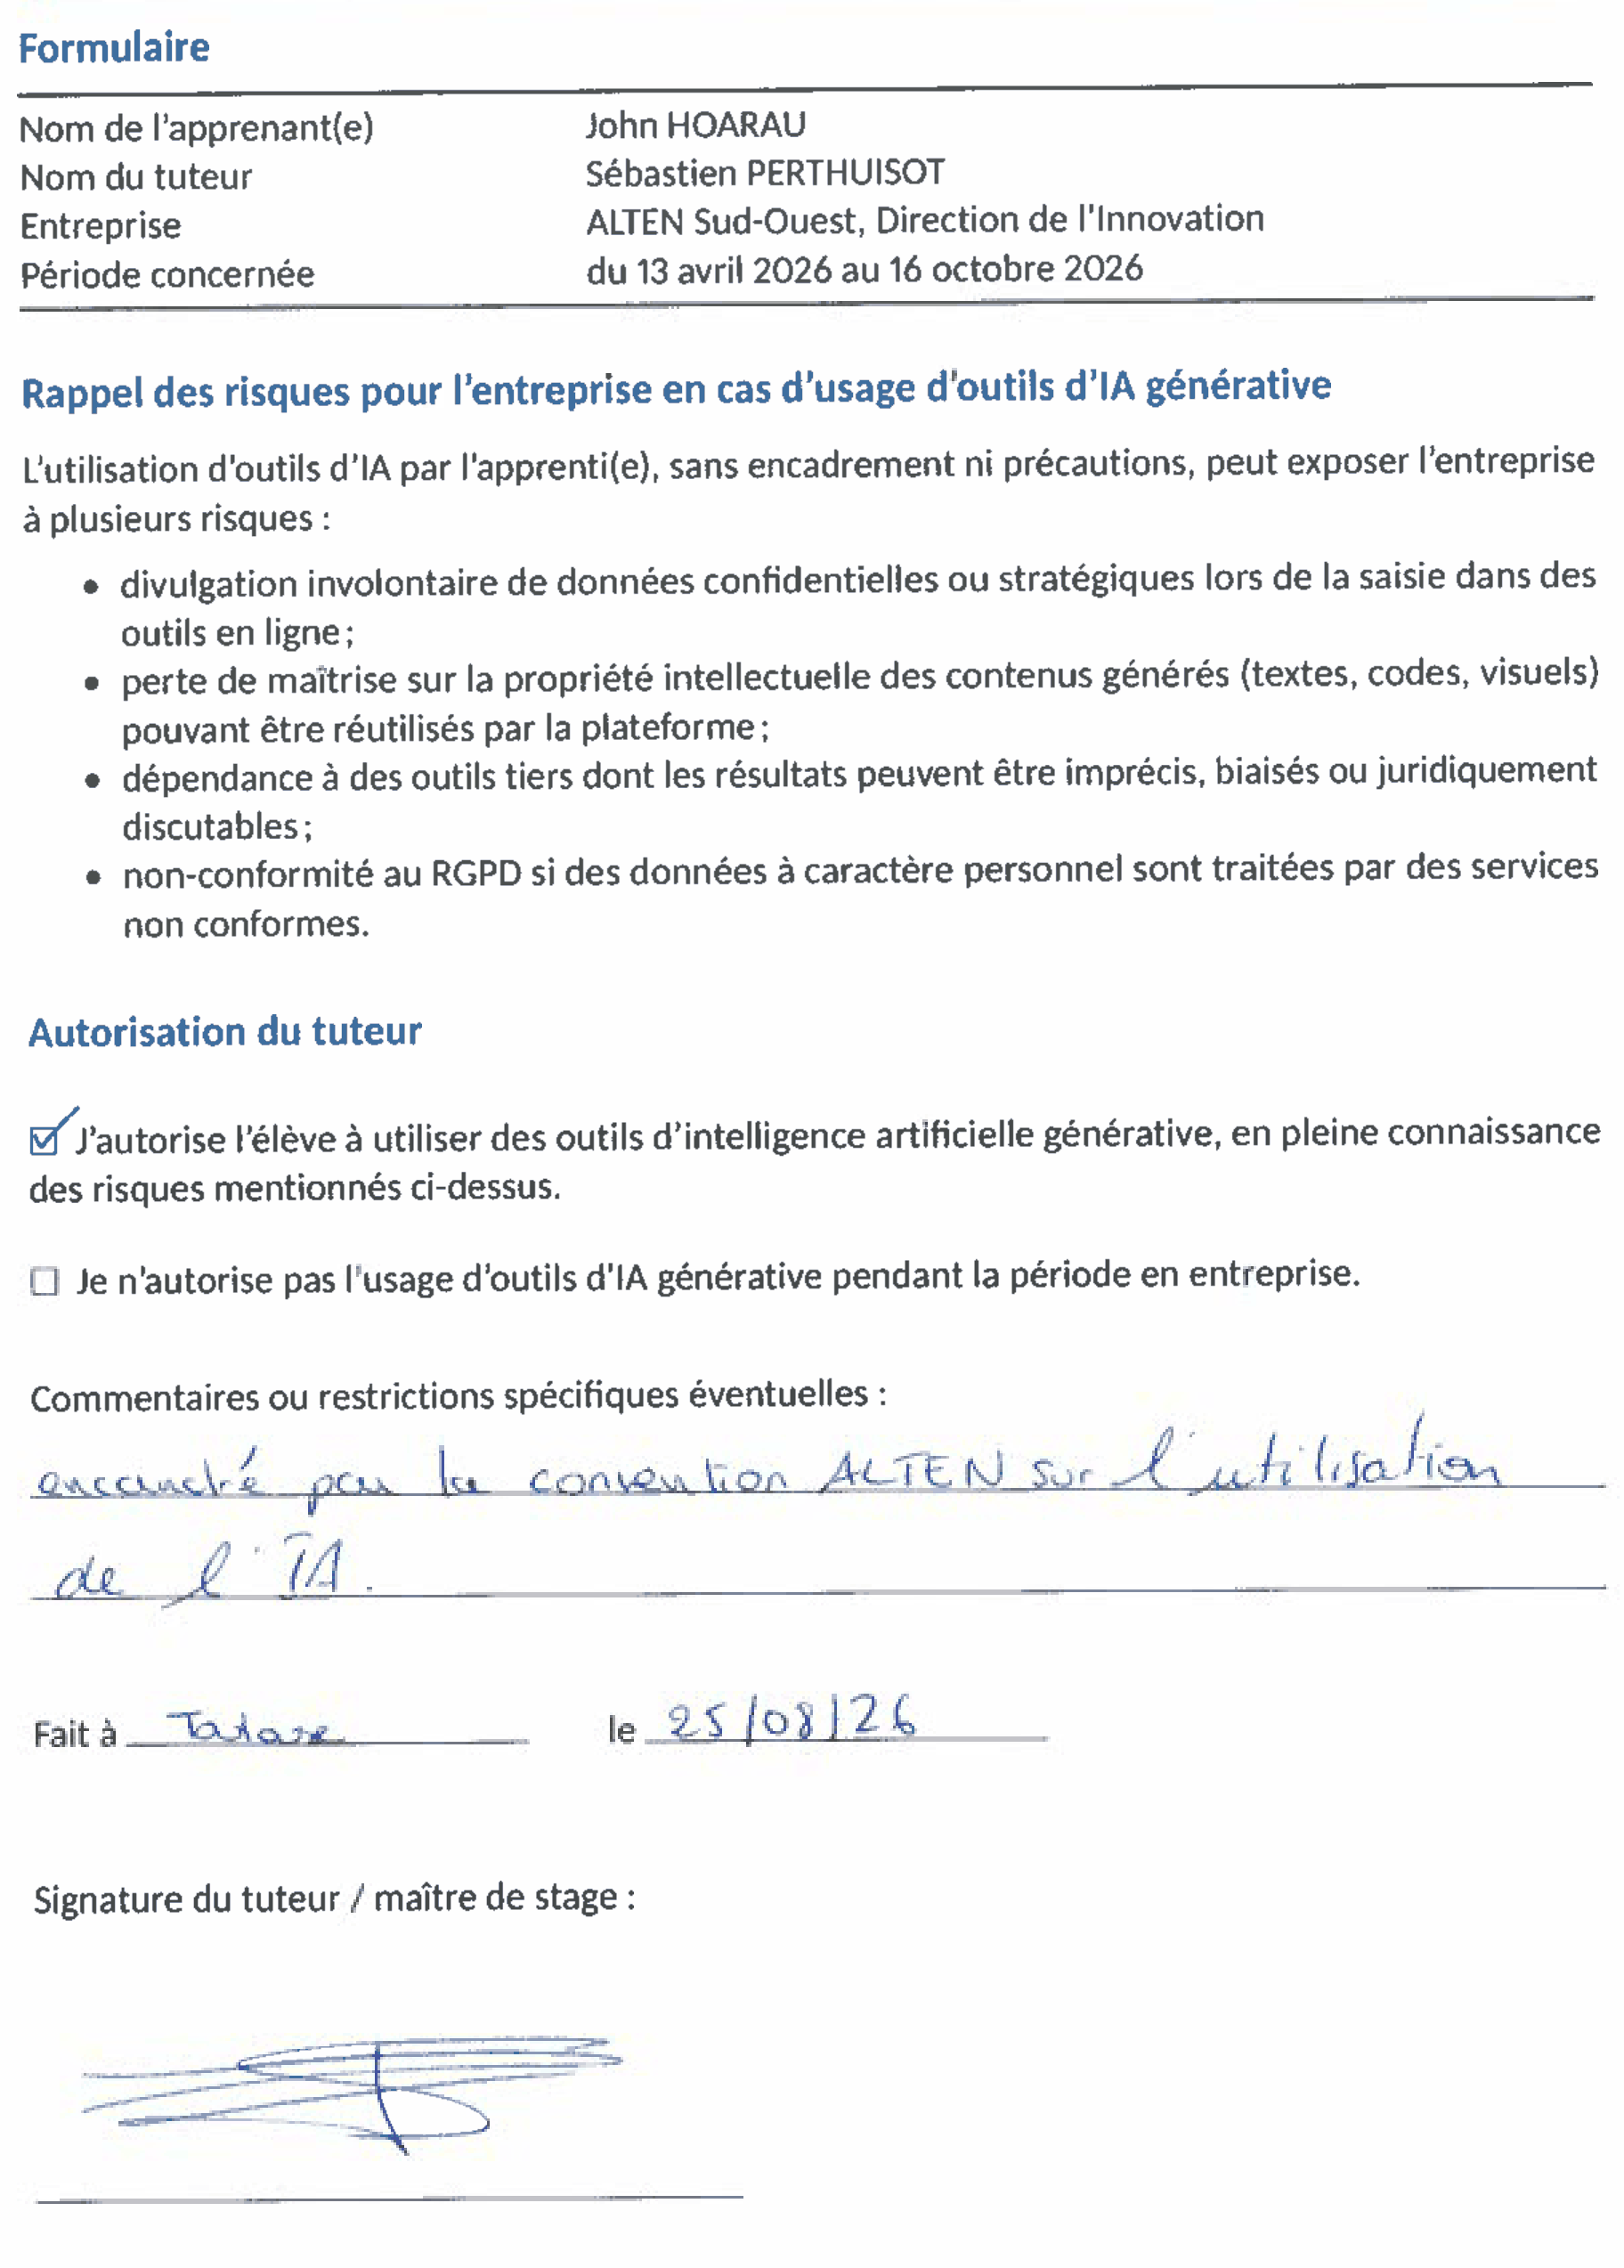
\includegraphics[width=0.88\linewidth]{Images/autorisation_ia_signee.png}
    \caption[Signed authorisation of AI use]{The authorisation form, signed.}
    \label{fig:autorisation_ia}
\end{figure}

\subsection*{Declared use of AI tools in this mission}

For transparency, and independently of the authorisation above, the use made of generative AI
during this internship is declared here in full.

Large language models were used in two distinct capacities, which should not be confused.

First, as an \emph{object of study}. The eight declarants of the experimental campaign
reported in Section~\ref{sec:realisation_experience} are language-model agents. This is an
experimental design choice, stated as such throughout the report, and its consequences for
the validity of the results are discussed rather than glossed over.

Second, as a \emph{writing aid}, for language correction and document formatting. Every
scientific claim, every numerical result and every interpretation in this report is my own,
and I am able to justify and explain each of them. Every figure was produced either by the
project's own code or by hand. No confidential ALTEN data was submitted to any external
service in the course of that assistance.
